\chapter {Miner\'ia y an\'alisis computacional de sentimientos}\label{Mineria}

Las opiniones son fuertemente influyentes sobre el comportamiento de las personas en la mayor\'ia de sus actividades. Nuestras creencias, decisiones y percepci\'on de la realidad est\'an condicionadas por la visi\'on que perciben las dem\'as personas en nuestro entorno. El \'area de estudio denominada ``an\'alisis de sentimientos'', conocida tambi\'en como ``miner\'ia de opiniones'' se ocupa de conceptos tales como opini\'on, sentimiento, actitud y evaluaci\'on (Liu, 2012).
\newline

En este cap\'itulo definimos el an\'alisis computacional como un Proceso de Descubrimiento de Conocimiento (KDD por sus siglas en ingl\'es, \textit{Knowledge Discovery in Databases}) y como un \'area de estudio del Procesamiento de Lenguaje Natural (PLN). Luego, se presentan las estrategias m\'as utilizadas en el campo, adem\'as de una breve descripci\'on de los trabajos similares m\'as recientes que utilizan dichas estrategias para la clasificaci\'on de sentimientos.

\section{Proceso de Descubrimiento de Conocimiento}
{Los datos son un conjunto discreto de hechos sobre ciertos eventos; los datos en s\'i no describen las condiciones de un evento, o posibles interpretaciones sobre el mismo, solamente sumarizan caracter\'isticas de dichos eventos. Su importancia radica en que sirven de materia prima en el proceso de generaci\'on de informaci\'on.
\newline

Los datos se convierten en informaci\'on cuando el receptor de dichos datos da un sentido o interpretaci\'on a los mismos, entonces podemos definir a la informaci\'on como un conjunto de datos con sentido, relevancia y prop\'osito para el receptor de los datos.
\newline

A partir de informaciones obtenidas, podemos definir KDD como el proceso no trivial de identificaci\'on de patrones v\'alidos, novedosos, potencialmente \'utiles y comprensibles en un conjunto de datos (Fayyad y otros, 1996). Este proceso puede ser aplicado al an\'alisis de sentimientos, puesto que buscamos identificar patrones en un lenguaje de entrada, que describan significativamente las opiniones del tal manera que podamos clasificarlas, por ejemplo, como ``positivas'' o ``negativas'' y presentarlas como informaci\'on generada.
\newline 

\begin{figure}[h]
\centering
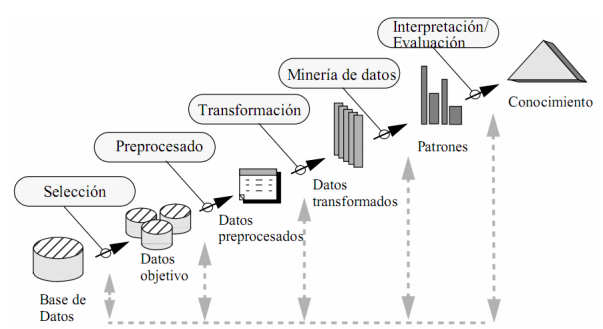
\includegraphics[width=1 \textwidth]{etapaskdd.png}
\caption{Etapas en el proceso de KDD (Fayyad y otros, 1996)}
\label{etapaskdd}
\end{figure}

En el proceso de KDD podemos distinguir una serie de etapas, como se puede observar en la Figura \ref{etapaskdd}, las cuales describimos a continuaci\'on:

\begin{itemize}

\item \textbf{Selecci\'on:} En esta etapa, el objetivo es escoger una fuente o conjunto de fuentes de datos como entrada. La selecci\'on de las fuentes se da a partir del an\'alisis previo del problema, de tal manera que los datos escogidos sean representativos del problema y resulten \'utiles para descubrir conocimiento. Adem\'as, se pueden generar nuevos repositorios de datos a partir del conjunto de datos seleccionado. La recolecci\'on, descripci\'on y exploraci\'on de datos son tareas comunes en esta fase del proceso.
\item \textbf{Preprocesamiento:} Esta etapa involucra operaciones de limpieza y preprocesamiento de los datos, as\'i como tambi\'en de integraci\'on de diferentes fuentes de datos. Algunas tareas comunes que efect\'uan en esta etapa son la selecci\'on de columnas para el an\'alisis de datos, la limpieza de los datos con ``ruido'', eliminaci\'on de registros repetidos y la definici\'on de acciones sobre los campos con registros nulos.
\item \textbf{Transformaci\'on:} La transformaci\'on de datos se efect\'ua con el objetivo de conseguir una caracterizaci\'on o representaci\'on de los datos, acorde a los objetivos planteados y, si es posible, reducir la cantidad de variables o atributos considerados, buscando un buen desempe\~no en las siguientes fases del proceso. Algunas tareas comunes en esta etapa son la discretizaci\'on de valores, agrupaciones por tipos y la reducci\'on de variables.
\item \textbf{Extracci\'on de Patrones:} En esta etapa se llevan a cabo trabajos de decisi\'on sobre los modelos y par\'ametros adecuados para obtener resultados coherentes y esperados sobre los datos, mapeando dichos modelos con las tareas adecuadas de miner\'ia para cada criterio u objetivo definido en el modelado. Las tareas comunes en esta fase del proceso son la clasificaci\'on, agrupaci\'on, asociaci\'on, visualizaci\'on y sumarizaci\'on de elementos, adem\'as de la detecci\'on de desv\'ios, estimaci\'on de valores, an\'alisis de relacionamiento, entre otras.
\item \textbf{Interpretaci\'on y Evaluaci\'on:} De acuerdo a los datos obtenidos, este paso primariamente implica una retroalimentaci\'on de las etapas previas con el fin de corregir errores o mejorar ciertos procedimientos. Adem\'as se realiza una visualizaci\'on sobre los patrones y modelos obtenidos de manera a comprender dichos resultados y extraer conocimientos. Durante las acciones de comprensi\'on y descubrimiento de conocimiento, se pueden presentar casos en los cuales los resultados generen conflictos con algunos conocimientos previos, por tanto la resoluci\'on de dichos inconvenientes puede implicar la modificaci\'on o actualizaci\'on de ciertos par\'ametros aplicados en pasos anteriores.

\end{itemize}

En las siguientes secciones, describimos algunas t\'ecnicas y caracter\'isticas utilizadas en las diferentes etapas descriptas, orientadas principalmente a la clasificaci\'on de textos. Adem\'as, en  el siguiente cap\'itulo se presenta una visi\'on general del proceso de descubrimiento en funci\'on al problema abordado.

\section{Preprocesamiento de entradas}

Este paso se efect\'ua previamente al de la estrategia de categorizaci\'on seleccionada, con el objetivo de limitar y refinar los espacios de b\'usqueda. En esta etapa del proceso se define cu\'ales entradas son relevantes y la disposici\'on m\'as eficiente en la que pueden ser introducidas al proceso de clasificaci\'on. Algunas t\'ecnicas de preprocesamiento son las siguientes:

\begin{itemize}

\item \textbf{Utilizaci\'on de n-gramas:} Los datos pueden ser introducidos en forma de n-gramas. Un n-grama consiste en una subsecuencia de n-elementos de una secuencia dada. En el estudio del lenguaje natural, se pueden introducir elementos de distinta granularidad, como letras, s\'ilabas o palabras. Sin embargo, en el an\'alisis de sentimientos, generalmente se utilizan las palabras. El caso base para la disposici\'on de los datos es la utilizaci\'on de las palabras como unigramas (subsecuencias de un elemento). Otra variante muy utilizada y que es objeto de varios experimentos con resultados positivos, es la introducci\'on de bigramas (subsecuencias de dos palabras) con el objetivo de aumentar la precisi\'on en la determinaci\'on de la polaridad de los textos, partiendo de la idea que con ellas se puede lograr una mejor evaluaci\'on de intensificadores, negadores y otros fen\'omenos gramaticales; por ejemplo, ``muy bueno'', ``no apto'' son bigramas significativos.

\item \textbf{Eliminaci\'on de stopwords:} Las \textit{stopwords} son un conjunto de palabras de uso muy frecuente y que son omitidas en el proceso de b\'usqueda, pues no representan entradas significativas (ru\'ido) para el an\'alisis pertinente; en este caso, cargas de polaridad. Varias de ellas son propias de la gram\'atica, como art\'iculos, nombres, preposiciones y otras categor\'ias l\'exicas; algunos ejemplos son: ``ac\'a'', ``ah\'i'', ``alg\'un'', ``del'', ``en'', entre otras. Otras palabras no significativas para el an\'alisis de sentimientos pueden ser aquellas relativas al dominio, pues son utilizadas de manera muy frecuente y tampoco implican orientaci\'on a alguna polaridad determinada; por ejemplo, en una cr\'itica de cine, estas palabras podr\'ian ser ``actor'', ``actuaci\'on'', ``sonido'', entre otras.

\item \textbf{Stemming:} El m\'etodo de \textit{stemming} consiste en obtener la ra\'iz sem\'antica de cada palabra con el objetivo de asociar las palabras con dicha ra\'iz. Con esto se logra reducir las formas derivadas de las palabras a su forma base. Por ejemplo, la ra\'iz del verbo ``aprender'' es ``aprend'', con lo que se logra asociar las conjugaciones de dicho verbo como ``aprende'', ``aprendo'', ``aprendiendo'', etc.

\item \textbf{Lematizaci\'on} La lematizaci\'on es similar al m\'etodo de \textit{stemming}, a diferencia de que \'este toma como ra\'iz de las palabras un subconjunto de letras de la misma; mientras que en el proceso de lematizaci\'on, se busca hallar el lema de una palabra, es decir su forma gen\'erica o como la encontrar\'iamos en un diccionario. Por ejemplo, mediante lematizaci\'on se puede lograr reducir la forma ``hice'' a su lema ``hacer'', mientras que esto no ser\'ia posible mediante \textit{stemming}.

\item \textbf{An\'alisis de estructuras gramaticales:} Llamada tambi\'en \textit{POS tagging} (por sus siglas en ingl\'es, \textit{``part-of-speech''}). Consiste en el etiquetado de las palabras seg\'un su categor\'ia gramatical, debido a que algunas de ellas son indicadoras m\'as relevantes de opini\'on. Ciertas categor\'ias como por ejemplo, los adjetivos o los adverbios, son m\'as descriptivas para detectar polaridad en una oraci\'on que los sustantivos, los verbos o los art\'iculos. Algunas aplicaciones de esta t\'ecnica son la asignaci\'on de pesos a las palabras por categor\'ia o bien la utilizaci\'on de las etiquetas mismas como atributos para un conjunto de entrenamiento.

\end{itemize}

Las t\'ecnicas citadas definen finalmente el modelo de entrada en un clasificador y la calidad del mismo. La aplicaci\'on de cada una de ellas debe ser analizada en funci\'on a las caracter\'isticas de la fuente y los datos de entrada disponibles.

\section{Estrategias basadas en l\'exicos}

En cualquier lenguaje, existen palabras com\'unmente utilizadas para expresar opini\'on o ``sentimiento'' con una orientaci\'on determinada respecto a una entidad en particular. Dicha orientaci\'on puede ser positiva o negativa; por ejemplo: ``bueno'', ``genial'' y ``espectacular'' son entradas positivas; mientras que ``malo'', ``p\'esimo'' y ``horrible'' son entradas negativas. Estas palabras, denominadas \textit{sentiment words} (SW, por sus siglas en ingl\'es) en conjunto conforman un l\'exico de sentimientos u opiniones. Para conformar dicho l\'exico, pueden ser tomados como fuentes distintos textos escritos, cuyos contenidos traten de evaluar o expresar opini\'on sobre alguna entidad, como por ejemplo cr\'iticas, libros, recetas, p\'aginas Web, entre otros.
\newline

Las SW podemos clasificar en palabras descriptivas y comparativas. Las palabras descriptivas expresan calificaci\'on sobre una entidad, tales como las citadas en el p\'arrafo anterior; mientras que las palabras comparativas establecen confrontaci\'on entre dos entidades, generando opiniones superlativas. Por ejemplo, en la oraci\'on ``El producto A es mejor que el producto B'' no se establece calificaci\'on positiva ni negativa para alguno de los productos, sino que solamente en comparaci\'on al producto B, el A es mejor. Esto no implica que ``mejor'' sea exclusivamente una SW comparativa para cualquier oraci\'on, sino que cumple tal funci\'on en el contexto dado.
\newline

En algunos l\'exicos, la orientaci\'on sem\'antica de las palabras es cuantificada generalmente por valores num\'ericos, que luego son introducidos en una funci\'on de puntuaci\'on, para determinar la polaridad de una opini\'on acerca de una entidad determinada. Dicha funci\'on var\'ia seg\'un el an\'alisis de distintos autores; as\'i como los criterios de cuantificaci\'on de las orientaciones sem\'anticas. En algunos trabajos, se limitan a asignar signos positivos y negativos (+1 y -1) a las palabras (Ding y otros, 2008); mientras que en otros, se emplea un intervalo m\'as amplio para obtener un mejor balance de la suma final de polaridades, como (Taboada y otros, 2011) que utilizan un intervalo de puntuaci\'on de -5 a +5. Estas puntuaciones, as\'i como las funciones definidas para el c\'alculo de polaridad, pueden influir en la precisi\'on de resultados logrados.
\newline

En (Liu, 2012) se identifican tres tipos de estrategia para compilar SW que conformen un l\'exico: la generaci\'on manual, la generaci\'on basada en un diccionario y la generaci\'on basada en un corpus.

\subsection{L\'exico generado manualmente}

Seguir esta estrategia implica un costo muy alto de trabajo y de tiempo, por tanto generalmente no es utilizada de manera exclusiva. Tiene su utilidad en combinaci\'on con estrategias automatizadas mediante tareas tales como una verificaci\'on final de palabras, puesto que con los m\'etodos automatizados se pueden generar errores.

\subsection{L\'exico basado en un diccionario}

La construcci\'on de un diccionario implica un listado de sin\'onimos y ant\'onimos para cada palabra. Un m\'etodo sencillo de generaci\'on es utilizar como semillas algunas SW, a partir de las cuales se pueden encontrar las dem\'as palabras del diccionario a partir de los sin\'onimos y ant\'onimos de las semillas. A medida que dichos sin\'onimos son agregados como nuevas palabras semilla, el diccionario va creciendo sucesivamente. Algunos trabajos que se ocupan de la generaci\'on de un diccionario son (Hu y Liu, 2004) y (Kim y Hovy, 2004).
\newline

La ventaja de utilizar un diccionario es que se puede encontrar f\'acil y r\'apidamente un gran n\'umero de SW con sus orientaciones sem\'anticas. A pesar de que la lista resultante puede incluir varios errores, es posible efectuar una verificaci\'on manual de limpieza para refinar el diccionario. Por otro lado, la principal desventaja es que la lista de palabras generadas en un diccionario son de prop\'osito muy general (no orientadas al dominio de aplicaci\'on) y dependientes del contexto. Esta dificultad puede tratada mediante la generaci\'on de un corpus.

\subsection{L\'exico basado en un corpus}

Esta estrategia fue mayormente aplicada frente a dos escenarios:

\begin{enumerate}
\item Dado un listado base de SW conocidas, de prop\'osito general, se descubren nuevas SW con sus orientaciones para un determinado dominio.
\item Adaptar un l\'exico de prop\'osito general a uno nuevo utilizando un corpus para aplicaciones de an\'alisis de sentimientos en el dominio.
\end{enumerate}
Construir un l\'exico de sentimientos para un dominio espec\'ifico puede no ser suficiente puesto que en el mismo dominio, una misma palabra puede ser positiva en un contexto, pero negativo en otro. Esta estrategia tambi\'en puede ser utilizada para construir un l\'exico de prop\'osito general en el caso que se encuentre disponible un corpus muy grande y diverso, pero para tal prop\'osito es m\'as efectiva la elaboraci\'on de un diccionario, puesto que el mismo ya est\'a compuesto por todas las palabras. Algunos trabajos que tratan la generaci\'on de un corpus son (Turney, 2002) y (Ding y otros, 2008). 

\subsection{Procesamiento de Lenguaje Natural}

Para extraer las opiniones o sentimientos (informaci\'on) a partir de un texto, el an\'alisis del mismo debe ser tratado como un problema de PLN. Como tal, debe considerar todos los aspectos de ella, como por ejemplo la desambiguaci\'on de palabras, las negaciones, intensificaciones, decrementaciones, entre otros.
\newline

El problema espec\'ifico de extracci\'on de opiniones, es un problema de PLN restringido puesto que no es necesario entender completamente la sem\'antica de cada oraci\'on o documento, mas debe interpretar \'unicamente ciertos aspectos de ellos, como los sentimientos positivos o negativos y las entidades o t\'opicos a los que se refieren. De todas maneras, existen tambi\'en otros problemas a\'un no resueltos de PLN que agregan ciertas dificultades al proceso de an\'alisis. A continuaci\'on, describimos algunos t\'opicos que representan tanto aspectos comunes como dificultades que son tratadas en los problemas de PLN.

\begin{itemize}

\item \textbf{Desambiguaci\'on de palabras:} Es un aspecto a llevar en cuenta, puesto que en el lenguaje de entrada pueden existir varias palabras que presentan polisemia, es decir cuando una  misma palabra representa diversos significados o acepciones. Esto conduce a que parte del problema considerado es identificar 	el sentido de la palabra dentro de una determinada oraci\'on o documento. Por ejemplo, la palabra ``vaya'' podr\'ia representar un verbo conjugado en presente subjuntivo, en modo imperativo, o incluso una interjecci\'on que denota admiraci\'on o asombro. La diferenciaci\'on de dichos significados es una capacidad humana sencilla, pero debe poder reproducirse adem\'as en los algoritmos de interpretaci\'on que sean desarrollados.
\item \textbf{Negaci\'on:} Es un elemento ling\"u\'istico que, como lo dice su nombre, se utiliza para negar una oraci\'on entera o alguna idea contenida en ella, mediante la utilizaci\'on de adverbios de negaci\'on. Tales adverbios pueden ser utilizados en distintos \'ordenes para referirse a la idea negada, es decir pueden aparecer antes, en medio o despu\'es de ellas. Algunos de estos adverbios de negaci\'on son ``no'', ``nunca'', ``jam\'as'', ``tampoco'', ``nada'' y ``negativamente''.
\item \textbf{Intensificaci\'on y Atenuaci\'on:} Consisten en la utilizaci\'on de ciertos adverbios como recursos ling\"u\'isticos para aumentar o disminuir la intensidad de alguna idea transmitida.  Algunos intensificadores de ejemplo son ``muy'', ``mucho'', ``demasiado'' y ``sobremanera'',  mientras que adverbios como ``poco'', ``menos'', ``solamente'', ``apenas'', ``justo'' son atenuadores.
\item \textbf{Palabras dependientes del contexto:} Son aquellas que no pueden ser definidas como orientadas positivamente o negativamente, sin conocer el dominio del tema que se est\'e abordando. Una palabra puede ser utilizada para referirse positivamente hacia una entidad en un determinado dominio; pero a la vez dicha palabra puede tener una implicancia negativa en un dominio diferente.
Por ejemplo, el adjetivo ``peque\~no'' puede ser visto como positivo refiri\'endose al tama\~no de un tel\'efono celular; o bien como negativo si es referido al tama\~no de una porci\'on de comida servida en un comedor.
\item \textbf{M\'ultiples orientaciones sem\'anticas:} Se presentan cuando se efect\'ua el an\'alisis de un texto que puede estar compuesto por varias oraciones, o bien varias ideas y \'estas pueden tener polaridades diferentes. La entidad a la que se est\'a refiriendo el texto puede ser la misma, pero distintas oraciones pueden referirse a diferentes caracter\'isticas de ella.  Por ejemplo, en la siguiente referencia a una c\'amara fotogr\'afica: ``La calidad de las im\'agenes es muy buena, pero la duraci\'on de la bater\'ia es muy corta.'', la opini\'on acerca de la caracter\'istica de calidad de las im\'agenes es positiva, mientras que la duraci\'on de la bater\'ia es vista negativamente. Ambas aparecen en una misma oraci\'on y adem\'as se refieren a la misma entidad, la c\'amara fotogr\'afica.
\item \textbf{Sarcasmo:} Es una figura que genera dificultades pues cuando se encuentra presente en una oraci\'on, pretende dar a entender lo contrario a lo que las palabras expresan. Es decir, se pueden encontrar varias palabras con orientaci\'on positiva, con la intenci\'on de manifestar negativismo de manera evidente, o viceversa.

\end{itemize}

El tratamiento de los problemas de PLN descriptos implica la caracterizaci\'on bien definida del lenguaje abordado pues deben ser tratados sus aspectos gramaticales, lo cual implica adem\'as que la constituci\'on del l\'exico debe ser lo m\'as detallada posible, puesto que la evaluaci\'on de nuevas instancias est\'a limitada a las palabras contenidas en \'el. Los trabajos citados en esta secci\'on tratan con mayor profundidad estos aspectos de los lenguajes.

\section{Estrategias basadas en aprendizaje de m\'aquina}

La estrategia basada en aprendizaje de m\'aquina, tambi\'en referida como estad\'istica o clasificadora de textos, consiste en entrenar un clasificador para categorizar elementos de entrada dentro de una clase perteneciente a un conjunto definido de clases; por ejemplo, de sentimientos positivos, negativos o neutrales. El objetivo es generalizar comportamientos a trav\'es de informaci\'on previamente recolectada, denominada conjunto de entrenamiento, en forma de ejemplos, que luego puedan ser utilizados para evaluar un texto en funci\'on a sus similaridades.
\newline

En t\'erminos generales un conjunto de entrenamiento, llamado en ingl\'es \textit{training set}, es un conjunto de datos que se utiliza para realizar pruebas iniciales sobre un modelo conceptual esperando conseguir una descripci\'on comprensible de dicho modelo y a partir del mismo, la generaci\'on de conocimiento. Adem\'as del conjunto de entrenamiento, es utilizado adem\'as un conjunto separado de datos denominado conjunto de evaluaci\'on (\textit{test set}), cuyos datos son diferentes a los utilizados en el conjunto de entrenamiento y cuya funci\'on es la de evaluar la efectividad del modelo creado ante instancias desconocidas por el mismo. A modo de ejemplo, si consideramos la Figura \ref{datasets}, existen dos clases diferentes: los c\'irculos rellenos y los c\'irculos vac\'ios. Las instancias representadas por dichas formas conforman el conjunto de entrenamiento, pues indicamos expl\'icitamente al clasificador a cu\'al de las clases pertenece cada una de ellas, de tal manera que el mismo tratar\'a de inferir sus caracter\'isticas y patrones. Luego, queremos clasificar nuevas instancias que no han formado parte de dicho conjunto y buscamos conocer a cu\'al de las clases pertenece cada una de ellas. Es as\'i que las instancias representadas por las $X$ conforman el conjunto de evaluaci\'on, las cuales seg\'un estimaci\'on del clasificador pertenecer\'an al conjunto de los c\'irculos rellenos o al de los vac\'ios.
\newline

\begin{figure}[h]
\centering
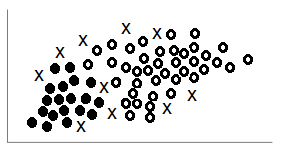
\includegraphics[width=0.5\textwidth]{datasets.png}
\caption{Conjuntos de entrenamiento y de evaluaci\'on en estrategias de aprendizaje de m\'aquina.}
\label{datasets}
\end{figure}

Podemos identificar dos tipos de aprendizaje en esta estrategia: supervisado y no supervisado. En un m\'etodo de aprendizaje supervisado, se produce una funci\'on de correspondencia entre las entradas y salidas deseadas del sistema; como por ejemplo clasificar las palabras seg\'un su categor\'ia l\'exica (verbos, sustantivos, adjetivos, etc), categor\'ia funcional (determinantes, cuantificadores, pronombres, etc) o su polaridad (positivas, negativas, neutras, etc), por lo que se necesita una base de conocimiento previamente elaborada, compuesta por ejemplos de etiquetados anteriores.
\newline

Los m\'etodos de aprendizaje no supervisado se llevan a cabo sobre conjuntos de ejemplos conformados \'unicamente por entradas al sistema; sin etiquetado de categor\'ias, a diferencia de los m\'etodos supervisados; por lo que el sistema debe tener capacidad de reconocimiento de patrones para etiquetar nuevas entradas.
\newline

Algunos clasificadores de aprendizaje de m\'aquina son Bayes Ingenuo (NB, por sus siglas en ingl\'es), Entrop\'ia M\'axima (ME, por sus siglas en ingl\'es) y M\'aquinas de Soporte Vectorial (SVM, por sus siglas en ingl\'es). En las siguientes subsecciones, definimos cada uno de ellos, utilizando el siguiente conjunto de variables:

\begin{itemize}
\item Un corpus de texto $C$, compuesto por una serie de documentos. La cantidad de documentos es irrelevante y cada uno de ellos es denominado $d$. 
\item Un conjunto de clases $\{c_{1},c_{2},\ldots,c_{n}\}$ definido.
\item Un conjunto de palabras que componen el corpus $C$. Todas las palabras $w$ que componen $C$ representan los atributos del conjunto de entrenamiento.
\end{itemize}

El objetivo es determinar a qu\'e clase $c$ pertenece cada documento $d$.

\subsection{Bayes Ingenuo} \label{bayes_sec}

El algoritmo basado en el teorema de Bayes, aplicado al an\'alisis de textos, consiste en clasificar cada palabra de acuerdo a la probabilidad de que pertenezca a un determinado grupo. Tales agrupaciones pueden estar determinadas por categor\'ias gramaticales o por polaridad. 
El an\'alisis de estructuras gramaticales permite, por ejemplo, establecer la probabilidad de que la palabra siguiente a un sustantivo sea un verbo; con el objetivo de determinar qu\'e influencia tiene una palabra en la polaridad de un texto. En este contexto, un adjetivo es m\'as descriptivo que un sustantivo para la inferencia del sentimiento transmitido en un texto. La asociaci\'on por polaridad, en cambio relaciona las palabras que componen una oraci\'on con el sentimiento que ellas en conjunto transmiten. Es decir, las palabras utilizadas en una oraci\'on considerada positiva son, con mayor probabilidad, palabras con asociaci\'on positiva para cualquier otra oraci\'on.
\newline

El clasificador de Bayes Ingenuo deriva del teorema de la probabilidad condicional de dos eventos aleatorios $A$ y $B$ enunciado por Thomas Bayes, donde ``la probabilidad del evento $A$ dado $B$'' est\'a expresado por la siguiente f\'ormula:
\newline \newline
$$P(A \, | \, B) \, = \, {P(A) \, P(B \, | \, A) \over P(B)},$$

Llevando dicho teorema al problema de la clasificaci\'on de textos y utilizando el conjunto de variables antes definido, el primer paso consiste en estimar la probabilidad $P(c)$ de cada clase $c$, dividiendo el n\'umero de palabras presentes en los documentos etiquetados en $c$ entre la cantidad total de palabras en el corpus $C$. Luego, la distribuci\'on de probabilidad $P(w \, | \, c)$ para todas las palabras por cada clase $c$ est\'a dada por la divisi\'on de la cantidad de ocurrencias de $w$ en los documentos etiquetados en $c$ entre la cantidad de palabras en $c$.
\newline

De esta manera, podremos asignar un valor num\'erico a un documento para cada una de las clases, para luego asociarlo a una de ellas. Dicho valor (Pang y otros, 2002) est\'a dado por:
\newline

$$ score(d \, | \, c) \, = \, P(c) \, * \, \prod_{i=1}^n \, P(w_{i} \, | \, c) $$

Luego, la estimaci\'on del modelo ser\'a de aquella clase cuyo valor de $score$ haya resultado mayor que el valor obtenido para las dem\'as clases.
\newline

A modo de ejemplo, en la Figura \ref{bayes} se puede ver que las instancias pueden ser clasificacadas en una de dos clases posibles. Para las instancias ya clasificadas, los c\'irculos rellenos representan a una clase, mientras que los vac\'ios representan a otra. Cuando se presenta una nueva instancia ($X$ en el ejemplo), el objetivo del clasificador consiste en estimar a cu\'al de las clases pertenece. Para el algoritmo de Bayes, como existe el doble de c\'irculos vac\'ios que de c\'irculos rellenos, es m\'as probable (dos veces m\'as) que la nueva instancia pertenezca a la clase de los c\'irculos vac\'ios. Si representamos gr\'aficamente una muestra, es trazado un c\'irculo que rodea a $X$ y a un cierto n\'umero de instancias clasificadas, independientemente a la clase a la que pertenezcan. Entonces, la intuici\'on del algoritmo consiste en calcular la probabilidad de que $X$ que sea un c\'irculo relleno, y la probabilidad de que sea un c\'irculo vac\'io mediante dicha muestra. Dichas probabilidades son calculadas seg\'un las f\'ormulas presentadas, de tal manera que el algoritmo estimar\'a que la nueva instancia pertenece a la clase con mayor valor de probabilidad.
\newline

\begin{figure}[h]
\centering
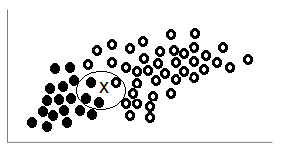
\includegraphics[width=0.5\textwidth]{bayes.png}
\caption{Clasificaci\'on de una nueva instancia mediante el algoritmo de Bayes Ingenuo.}
\label{bayes}
\end{figure}

La dificultad en la aplicaci\'on de este algoritmo es que est\'a cimentado en la hip\'otesis de que las variables evaluadas son independientes entre s\'i (visto en la multiplicaci\'on de los valores de $P(w_{i} \, | \, c)$ en la definici\'on de $score$); y como la gram\'atica es por el contrario, dependiente del contexto, muchas entradas son clasificadas err\'oneamente, originando los fen\'omenos conocidos como ``falsos positivos'' o ``falsos negativos'' si tratamos la polaridad. Sin embargo, los resultados pueden ser a\'un muy positivos con la determinaci\'on de un buen conjunto de entrenamiento.

\subsection{Entrop\'ia M\'axima}

El clasificador por entrop\'ia m\'axima trata de generar informaci\'on reduciendo el sesgo al m\'inimo posible. El principio fundamental del algoritmo es que son preferidas las distribuciones uniformes que satisfacen adem\'as todas las restricciones del problema (Nigam y otros, 1999). Dichas restricciones que caracterizan al modelo, son derivadas de los datos etiquetados del conjunto de entrenamiento.
\newline

El algoritmo trata de identificar las caracter\'isticas que definen una clase, definiendo un modelo que englobe las reglas que puedan ser inferidas del conjunto de entrenamiento. Luego, estima un valor esperado para cada una de las clases definidas, de manera a tratarlos como restricciones en el modelo de distribuci\'on (Lee y Renganathan, 2011).
\newline

A diferencia del algoritmo de Bayes Ingenuo, no asume la independencia entre variables. En cambio, el modelo busca mediante las restricciones mencionadas, maximizar la adherencia entre atributos en relaci\'on a alguna clase, de tal manera que una nueva entrada ser\'a categorizada dentro una clase cuanto menos caracter\'isticas extr\'insecas a su definici\'on contenga.
\newline

Nigam y otros (1999) definen la probabilidad $P(c \, | \, d)$ de cada clase de la siguiente manera:
\newline

$$ P(c \, | \, d) \, = \, {1 \over Z(d)} \, exp \, 
\left(
\sum_{i} \lambda_{i}F_{i}(d,c)
\right) ,$$

Con la siguiente definici\'on de par\'ametros:

\begin{itemize}
\item Cada $F_{i}(d,c)$ es un atributo
\item $\lambda_{i}$ es el par\'ametro a ser estimado. Es un indicador de peso; es decir, un valor mayor indica que $F_{i}$ es un indicador m\'as relevante para la clase $c$.
\item $Z(d)$ es una funci\'on de normalizaci\'on para definir una probabilidad apropiada, dada por la siguiente expresi\'on:
$$
Z(d) = \sum_{c} \, exp \, \left( \sum_{i} \lambda_{i}F_{i}(d,c)  \right)
$$
\end{itemize}

La b\'usqueda de $\lambda_{i}$ se realiza por medio de algoritmos de b\'usqueda iterativa definidos seg\'un el modelo, como por ejemplo el m\'etodo de Ascenso de Colinas o el de Temple Simulado.
\newline

Si utilizamos el mismo ejemplo mostrado en el algoritmo de Bayes, podemos observar en la Figura \ref{entropy} la separaci\'on trazada mediante la funci\'on de Entrop\'ia M\'axima. Este algoritmo esboza una separaci\'on de clases por atributo, buscando la mejor diferenciaci\'on posible. Si consideramos la distribuci\'on de datos seg\'un el eje de abscisas y seg\'un el eje de ordenadas, se puede apreciar que est\'an mejor separados en el segundo caso (demarcado por la l\'inea punteada), de modo que el atributo representado en dicho eje ser\'a el primer atributo de decisi\'on para el clasificador, de manera similar a un \'arbol de decisi\'on.
\newline

\begin{figure}[h]
\centering
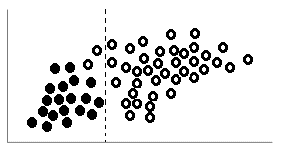
\includegraphics[width=0.5\textwidth]{entropy.png}
\caption{Separaci\'on de clases a trav\'es del algoritmo de Entrop\'ia M\'axima.}
\label{entropy}
\end{figure}

Las dificultades que pueden presentarse con el m\'etodo de entrop\'ia m\'axima son la facilidad con la que se presentan casos de \textit{overfitting} (sobreentrenamiento del algoritmo con los datos de entrada dados, que produce p\'erdida de generalizaci\'on para datos nuevos) y el tiempo que pueda emplearse en la determinaci\'on de los pesos puesto que las iteraciones para calcularlos pueden llegar a ser infinitas.
\newline

\subsection{M\'aquinas de Soporte Vectorial} \label{sec:svm}

Para describir el algoritmo de M\'aquinas de Soporte Vectorial (SVM, por sus siglas en ingl\'es), es precisa la definici\'on de una serie de ideas preliminares, como los problemas de clasificaci\'on lineal, los hiperplanos y los m\'argenes geom\'etricos.
\newline

Podemos definir los datos en los problemas de clasificaci\'on lineal como aquellos que est\'an identificados con una de dos posibles clases, por ejemplo, positivos o negativos. Es as\'i que dentro de un conjunto de datos se tienen vectores $X$ y clases $Y$, representados por la forma $(X_{i},Y_{i})$ e interpretados como el $i$-\'esimo dato dentro del conjunto, asociado a una de las clases definidas. En los problemas de clasificaci\'on lineal se utilizan los hiperplanos, los cuales son superficies que dividen al espacio de distribuci\'on en dos partes.
\newline

La idea detr\'as del SVM es la siguiente. Dado un conjunto de vectores de dos clases distintas, distribuidos en un plano $n$-dimensional; se busca encontrar una superficie o hiperplano que logre separar ambas clases con la mayor distancia posible respecto a los vectores de clases distintas que se encuentran a una distancia m\'inima.
\newline

\begin{figure}[h]
\centering
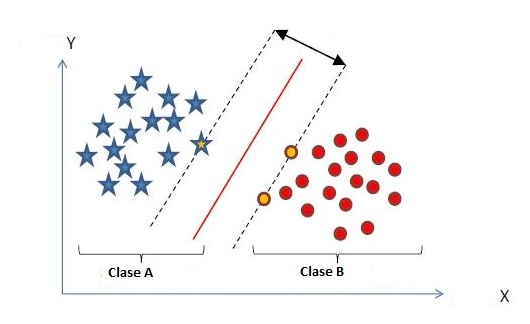
\includegraphics[width=0.7\textwidth]{separacion_hiper.png}
\caption{Separaci\'on de clases mediante un hiperplano en SVM.}
\label{svm:separacion_hiper}
\end{figure}

Como se muestra en la Figura \ref{svm:separacion_hiper}, el hiperplano logra realizar una separaci\'on entre vectores de clases distintas, a la mayor distancia posible entre los vectores de clase $A$ y $B$ m\'as pr\'oximos entre s\'i. En muchos casos, no puede ser dibujado un hiperplano entre vectores de clases distintas, debido a la distribuci\'on de dichos vectores; es entonces que se realiza un mapeo de los vectores en dimensiones superiores, de manera a encontrar el hiperplano que pueda realizar la divisi\'on entre las clases de vectores. Este mapeo, que se puede observar en la Figura \ref{svm:kernel}, es efectuado mediante una funci\'on denominada \textit{kernel}.
\newline

\begin{figure}[h]
\centering
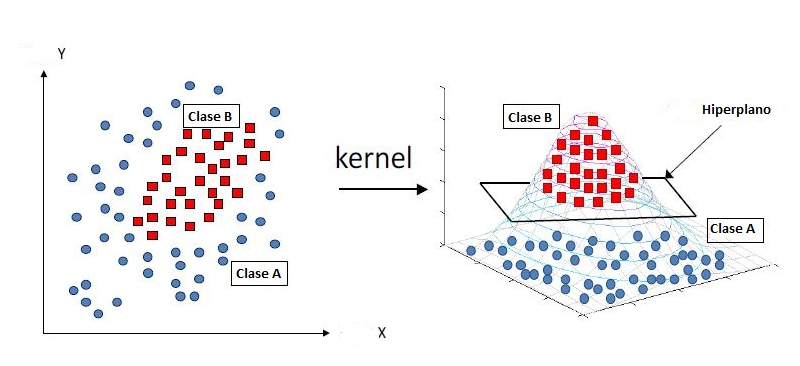
\includegraphics[width=0.9\textwidth]{kernel.png}
\caption{Mapeo de vectores en dimensiones superiores mediante una funci\'on kernel en SVM.}
\label{svm:kernel}
\end{figure}

En los problemas de clasificaci\'on lineal se cuenta con la funci\'on $f(x) \, = \, w^{T}x \, + \, b
$, en la cual el vector $w$ es conocido como el vector peso o vector director del plano, y la $b$ es el sesgo.
\newline

Considerando el caso que $b \, = \, 0$, los puntos en $x$ tales que $w^{T}x \, = \, 0$, ser\'an puntos en los cuales $x$ es perpendicular a $w$ y pasan por el origen, formando una l\'inea (para el caso de dos dimensiones) o un plano (para el caso de tres dimensiones) y m\'as generalmente, un hiperplano.
\newline

El valor de $B$ se encarga de trasladar al hiperplano alej\'andolo de su origen a trav\'es del vector $w$, entonces se tiene que el hiperplano $f(x) \, = \, w^{T}x \, + \, b \, = 0$ divide el espacio en dos a partir del valor que se obtenga de la funci\'on $f(x)$.
\newline

En una clasificaci\'on lineal donde se tienen distribuciones de puntos en el plano y se representan clases diferentes mediante dichos punto, buscando generalizaci\'on en los resultados la idea es establecer un hiperplano en medio de las clases de manera a diferenciarlas, m\'as precisamente, establecer el hiperplano a una distancia m\'axima de los puntos m\'as cercanos de cada clase, a esta distancia se la conoce como \textbf{margen}.
\newline

Teniendo un conjunto de puntos, al que llamamos conjunto $C$, se puede decir que tiene una \textbf{envoltura convexa} siempre y cuando exista un conjunto convexo que contenga a todos los puntos de $C$, y es expresado como $conv(C)$. Como se denota en la Figura \ref{svm:est_convexa}, el conjunto de puntos de la izquierda tiene una envoltura convexa que se indica a su derecha, conteniendo a todos los puntos del conjunto.

\begin{figure}[h]
\centering
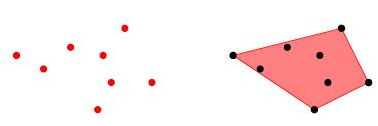
\includegraphics[width=0.7\textwidth]{est_convexa.png}
\caption{Envoltura convexa de un conjunto de puntos.}
\label{svm:est_convexa}
\end{figure}

Tomando como ejemplo la Figura \ref{svm:envoltura_puntos}, la envoltura convexa de un conjunto de puntos puede ser representada por la combinaci\'on de puntos que se encuentran en los extremos de dicha envoltura $\{e_{1},e_{2},\ldots,e_{n}\}$ o bien, puntos que determinan el per\'imetro de la figura que forman.

\begin{figure}[h]
\centering
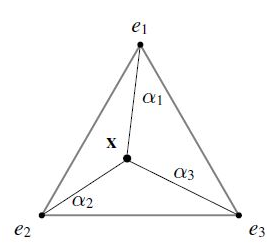
\includegraphics[width=0.4\textwidth]{envoltura_puntos.png}
\caption{Combinaci\'on de puntos de una envoltura convexa.}
\label{svm:envoltura_puntos}
\end{figure}

Esta combinaci\'on de puntos de extremos cuentan con pesos, representados por $\alpha$, que son la distancia al baricentro de la figura que forman. A estos valores se los conoce como coordenadas baric\'entricas de la envoltura convexa, y tienen la propiedad de que la sumatoria de los pesos es siempre igual a 1, como se expresa en la siguiente formulaci\'on:
$$
x \, = \, \sum_{i=1}^n \alpha_{i}e_{i}	\quad	y	\quad
\sum_{i=1}^n \alpha_{i} \, = 1
$$

Con las definiciones, se puede decir que el margen de un hiperplano, dadas dos clases de datos en la distribuci\'on ${X_{1},X_{2}}$, es la distancia m\'inima existente entre dicho hiperplano y los puntos de las clases definidas:
$$
margen \ = \ \min_{x \in x_{1} \cup x_{2}} \, d(x,H)
$$
o, lo que es equivalente, la distancia m\'inima existente entre el hiperplano y las coordenadas baric\'entricas de cada envoltura convexa de cada clase dada, lo cual puede formularse de la siguiente manera:
$$
margen \ = \ \min \lbrace d(H,conv(X_{1})),d(H,conv(X_{2})) \rbrace
$$

En cada envoltura convexa existen coordenadas baric\'entricas que se encuentran a menor distancia del hiperplano. A los puntos que cumplen esta propiedad de distancia m\'inima al hiperplano se los conoce como \textbf{vectores de soporte}.

\begin{figure}[h]
\centering
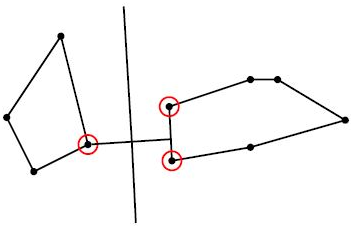
\includegraphics[width=0.4\textwidth]{coordenadas_bari.png}
\caption{Vectores de soporte en una envoltura convexa.}
\label{svm:coordenadas_bari}
\end{figure}

Como se observa en la Figura \ref{svm:coordenadas_bari}, pueden existir al menos dos vectores de soporte, uno por cada clase, a cada lado del hiperplano. As\'i tambi\'en, si existen cambios en los vectores de soporte, dichos cambios repercutir\'an en la clasificaci\'on y la ubicaci\'on del hiperplano para una determinada distribuci\'on.
\newline

Delineadas las ideas preliminares, podemos definir entonces a las SVM para el caso de una clasificaci\'on lineal. Como se estableci\'o previamente, se considera que existe un conjunto de datos $\lbrace (X_{1},Y_{1}), \, \ldots, \, (X_{m},Y_{m}) \rbrace$, para los cuales las $Y_{i}$ pertenecen al dominio de $\lbrace -1, \, -1 \rbrace$ para las diferentes clases con que se cuenta, y las $X_{i}$ pertenecen al espacio $R$ dimensional. Supongamos que tenemos un hiperplano que divide los puntos en ambas clases establecidas, es decir, valores de $Y \, = \, -1$ por un lado y valores de $Y \, = \, 1$ por el otro, y los puntos $X$ que se encuentran sobre el hiperplano cumplen con la siguiente funci\'on:
$$
w \, . \, x \ + \ b \ = \ 0
$$ 
donde $w$ es la recta normal al hiperplano, $x$ es un punto en el hiperplano y $b$ es el sesgo, que mueve el hiperplano a trav\'es del vector $w$, por lo que se conoce el valor de dicha distancia perpendicular del hiperplano a su origen, representado por ${|b| \over ||w||}$, donde $||w||$ es la Distancia Eucl\'idea del vector $w$.
\newline

En la distribuci\'on de puntos y el hiperplano definido, la distancia m\'as corta entre el hiperplano y uno de los puntos de una clase dentro de la distribuci\'on, puede ser definida como una distancia $d$(clase). Entonces si tenemos una clase $A$, la distancia m\'as cercana del hiperplano a un ejemplo, ser\'ia $d(A)$ (Alves Kaestner, 2013).
\newline

Por estos puntos cercanos al hiperplano se pueden trazar otros hiperplanos que tendr\'an restricciones con respecto a la clase a la que corresponden, de manera  que se puede tener la siguiente formulaci\'on (Burges, 1998):
$$
x_{1} \, . \, w \, + \, b \, \ge \, +1 \quad para \ y_{i} \, +1 $$
$$
x_{1} \, . \, w \, + \, b \, \le \, +1 \quad para \ y_{i} \, -1
$$
Estas formulaciones pueden ser combinadas en la siguiente igualdad:
$$
y_{1}(x_{1} \, . \, w \, + \, b) \, - \, 1 \, \ge \, 0	\quad \forall i
$$
Con estos valores, observamos que las distancias eucl\'ideas correspondientes a cada formulaci\'on ser\'ian: 
$$ 
m_{+} \, = \, {|1 \, + \, b| \over ||w||} \quad para \, el \, primer \, hiperplano $$
$$ 
m_{-} \, = \, {|-1 \, + \, b| \over ||w||} \quad para \, el \, segundo \, hiperplano
$$
Como ambos hiperplanos son paralelos y sus distancias $d(+,-)$ son iguales en m\'odulo pero a distintos lados del hiperplano central, la idea es que dicho hiperplano central sea el bisector de la distancia existente entre los hiperplanos paralelos, positivo y negativo. Entonces, la distancia entre los hiperplanos paralelos estar\'a dada por (Alves Kaestner, 2013):
$$
|m_{+} \, - \, m_{-}| \ = \ {2 \over ||w||}
$$
as\'i que minimizando $||w||$ estar\'iamos maximizando el margen que existe entre los hiperplanos paralelos.
\newline

Entonces, la funci\'on del algoritmo de SVM est\'a dada de la siguiente forma:
$$
\min {1 \over 2} \, ||w||^{2} \quad sujeto \, a \quad \lbrace \, y_{i}(w' \, . \, x_{i} \, - \, b) \ge 1
$$

Luego, es necesario pasar a una formulaci\'on lagrangiana del problema, ya que se sustituir\'a dicha formulaci\'on por otra con multiplicadores de Lagrange para que la misma provea una mayor facilidad de manejo computacional (Burges, 1998).
\newline

La regla para introducir los multiplicadores de Lagrange es que para restricciones de la forma $ c>=0$ las ecuaciones que las definen se multiplican por multiplicadores de Lagrange positivos y se restan de la funci\'on objetivo. Para el caso de las restricciones de la forma $C=0$, los multiplicadores no tienen restricciones. Teniendo en cuenta esto, la anterior funci\'on quedar\'ia de la siguiente forma:
$$
L_{P} \, = \, {1 \over 2} ||w||^{2} \ - \ \sum_{i=1}^N \alpha_{i} z_{i} (w \, . \, x_{i} \, + \, b) + \sum_{i=1}^N \alpha_{i}
$$

Ahora se trata de minimizar $L_{P}$ con respecto a $w$, $b$ y a la vez exigir que las derivadas de $L_{P}$ con respecto a todos los $\alpha$ se anulen; todo esto sujeto a restricciones de $\alpha_{i}>=0$ (Burges, 1998). Entonces, si se efect\'uan las derivadas de $L_{P}$ con respecto a $w$ y $b$, y las mismas se establecen a cero, se tiene:
$$
{\partial L_{P} \over \partial w} \ = \ 0 \quad \rightarrow \quad w \ = \ \sum_{i=1}^N \alpha_{i} z_{i} x_{i}$$
$$
{\partial L_{P} \over \partial b} \ = \ 0 \quad \rightarrow \quad \sum_{i=1}^N \alpha_{i} z_{i} \, = \, 0
$$
Estos valores se sustituyen en la formulaci\'on de $L_{P}$, siendo:
$$
L_{D} \ = \sum_{i=1}^N \alpha{i} \ - \ {1 \over 2} \sum_{i,j=1}^N \alpha_{i} \alpha_{j} z_{i} z_{j} x_{i} x_{j}
$$
la formulaci\'on dual del algoritmo de SVM para problemas lineales. De esta manera se observa que la funci\'on del problema lineal del SVM se resuelve maximizando $L_{P}$ o minimizando $L_{D}$ (Burges, 1998).
\newline

Ha sido demostrado varias veces que este m\'etodo es altamente efectivo para la categorizaci\'on de textos, obteniendo generalmente mejores resultados que la t\'ecnica de Bayes (Joachims, 1998; Pang y otros, 2002; Kennedy e Inkpen, 2006).

\section{M\'etricas de evaluaci\'on}

La evaluaci\'on de la clasificaci\'on se efect\'ua primariamente con el objetivo de comparar el desempe\~no de distintos sistemas o m\'etodos entre s\'i. La relevancia y utilidad de los resultados obtenidos prevalecen sobre los tiempos y espacios de respuesta cuando evaluamos una estrategia de an\'alisis de textos. No existe un \'unico criterio que permita determinar que un m\'etodo es mejor que otro; por ello, existen diversas m\'etricas para medir la efectividad de la informaci\'on obtenida del an\'alisis.
\newline

Las m\'etricas que presentamos en esta secci\'on est\'an basadas en la matriz de confusi\'on o de clasificaci\'on. Dicha matriz contrasta la estimaci\'on del modelo clasificador para un elemento dado, con la clase real asociada a dicho elemento.
\newline

Dado un conjunto de datos $E$, donde cada elemento $e$ puede ser representado como un vector $< e_1, e_2, \dots, e_n >$ de $n$ atributos, y un conjunto de clases $C$; cada vector $e \in E$ tiene una clase $c \in C$ asociada. La clasificaci\'on consiste en asignar una clase $c \in C$ para cada elemento $e \in E$, y el objetivo es cuantificar la efectividad de dichas asignaciones. Para dicho efecto, las filas de la matriz de confusi\'on representan las clases reales a la que pertenecen cada uno de los elementos y las columnas representan a la predicci\'on del modelo clasificador, como se observa en el Cuadro \ref{matrizconfusion}.
\newline

\begin{table}[htb] 
\centering

$
\begin{array}{|c|c|c|c|}
      \hline
         				& \mathbf{Clase_1}	& \mathbf{Clase_2}	& \mathbf{Clase_n}	\\
      \hline
      \mathbf{Clase_1}  & V	Clase_1	& F Clase_2	& F Clase_n	\\
      \hline
      \mathbf{Clase_2} 	& F Clase_2 & V Clase_2 & F Clase_n	\\
      \hline
      \mathbf{Clase_n}	& F Clase_n	& F	Clase_2	& V Clase_n	\\
      \hline
\end{array}
$
\caption{Matriz de confusi\'on o de clasificaci\'on}
\label{matrizconfusion}
\end{table}

Referenciando los sub\'indices de filas y columnas como $[i,j]$, una entrada Verdadera representa un acierto, es decir si el clasificador ha determinado que un elemento $e$ pertenece a la $Clase_j$ y dicho elemento efectivamente est\'a asociado a la $Clase_j$; mientras que una entrada Falsa representa un error de clasificaci\'on, es decir que el elemento $e$ no pertenec\'ia efectivamente a la $Clase_j$.
\newline

Definimos a continuaci\'on algunas m\'etricas de evaluaci\'on, en cuyas definiciones referenciamos a los aciertos y errores con el sub\'indice de la fila $i$ a la que pertenecen en la matriz de confusi\'on, como Verdadero de la $Clase_i$ o Falso de la $Clase_i$. 

\subsection{Precisi\'on}

La precisi\'on respecto a la $Clase_i$ indica el n\'umero de predicciones correctas sobre el total de predicciones de dicha clase. Es decir, indica la probabilidad de que un elemento $e$ pertenezca realmente a la $Clase_i$ dado que fue identificado como tal por el clasificador. Est\'a dado por la proporci\'on de verdaderos de la $Clase_i$ en relaci\'on a los totales identificados como de dicha clase:
\newline

$$ Precisi\acute{o}n = {V Clase_i \over V Clase_i + F Clase_i} $$ 
\newline

Si utilizamos el escenario de un tirador disparando a un blanco a modo de ejemplo, podemos decir que el mismo es preciso si las marcas de sus disparos son cercanas entre s\'i, independientemente a que ellas se encuentren cerca o lejos del blanco central.

\subsection{Exhaustividad}

La exhaustividad respecto a la $Clase_i$ indica el n\'umero de predicciones acertadas como $Clase_i$ sobre el total de elementos que realmente pertenecen a dicha clase. Es la probabilidad de que un elemento $e$ que pertenece realmente a la $Clase_i$ sea clasificado como tal. Est\'a dado por la raz\'on entre los verdaderos de la $Clase_i$, sobre los elementos reales de la $Clase_i$, en la matriz de confusi\'on dados por la suma de los verdaderos de la $Clase_i$ m\'as los falsos de las dem\'as clases.
\newline

$$ Exhaustividad = { V Clase_i \over V Clase_i + F Clase_j } \quad donde \quad j \in \lbrace 1,2,\dots,n \rbrace \quad con \quad j \ne i $$
\newline

Recurriendo nuevamente como ejemplo al escenario del tiro al blanco, la exhaustividad s\'i se refiere efectivamente a la cantidad de tiros que dieron en el blanco central de la diana.

\subsection{Medida-F}
La Medida-F relaciona las medidas de precisi\'on y exhaustividad mediante una media con el mismo peso para ambas. Es conocida tambi\'en como $F_1$ por la uniformidad de los pesos.
\newline

$$ Medida-F = {2 \, \times Precisi\acute{o}n \, \times \, Exhaustividad \over Precisi\acute{o}n \, + \, Exhaustividad}$$
\newline

Esta medida es muy utilizada en los problemas de clasificaci\'on pues las medidas anteriores describen propiedades distintas del clasificador y son relativas al problema tratado. Entonces, la medida-F proporciona una cuantificaci\'on general que permite evaluar la calidad del modelo clasificador.

\section{Propuestas similares}

En esta secci\'on, describimos algunas propuestas publicadas recientemente, con el fin de conocer los \'ultimos enfoques presentados que fueron utilizados efectivamente para an\'alisis de sentimientos. Seleccionamos preferentemente trabajos con similitudes tales como el idioma abordado (espa\~nol o enfoques multiling\"ues), las fuentes de datos (mediadores de redes sociales) o las estrategias utilizadas (mediante l\'exicos o aprendizaje de m\'aquina).
\newline

Moreno-Ortiz y P\'erez Hern\'andez (2013) presentan una propuesta basada en un l\'exico para categorizar textos cortos, al principio en cuatro categor\'ias de polaridad (positivos, negativos, neutros o sin polaridad) y luego agregando dos categor\'ias m\'as (muy positivos y muy negativos). El c\'alculo de polaridad est\'a centrado principalmente en dos valores num\'ericos denominados \textit{Global Sentiment Value} (GSV) y \textit{Affect Intensity} (AI); el primero, es un valor dentro de la escala de 0 a 10 asignado a sentimientos de acuerdo a una entrada de texto a partir del AI, el cual modula el GSV para reflejar el porcentaje de palabras con cierta carga de sentimientos. El AI no es un contador de palabras por polaridad, sino que de segmentos de texto que correspondan a unidades l\'exicas, definido como el porcentaje de segmentos que presentan determinada carga de polaridad, representando un paso intermedio para el ajuste de los l\'imites superior e inferior de las valencias relacionadas con el grado de sentimientos. Finalmente, concluyen que los valores de GSV se ven fuertemente afectados por la escasez de segmentos l\'exicos en los mensajes de Twitter; que la tendencia de la herramienta utilizada es la asignaci\'on de clasificaciones promedio, reflejada en la baja precisi\'on para las dos \'ultimas categor\'ias agregadas como ``extremos'' y adem\'as, que no es recomendable la diferenciaci\'on entre la categor\'ia de neutro con la de ausencia de polaridad.
\newline

Vilares, Alonso y G\'omez-Rodr\'iguez (2013) presentan una propuesta basada en un l\'exico complementada con an\'alisis sint\'actico de dependencias, para tratar las construcciones ling\"u\'isticas e identificar los elementos implicados en las oraciones. El preprocesamiento, fundamental para el posterior an\'alisis sint\'actico, implica la unificaci\'on de expresiones compuestas que act\'uan como una sola unidad de significado, la normalizaci\'on de signos de puntuaci\'on y la segmentaci\'on del texto en oraciones, adem\'as de la separaci\'on de ellas en \textit{tokens} de palabras y signos de puntuaci\'on. El \'arbol de dependencias creado permite identificar relaciones binarias entre los elementos de una oraci\'on, en el cual cada v\'inculo constituye una funci\'on sint\'actica que relaciona dos t\'erminos. En cuanto al an\'alisis sem\'antico, la propuesta se basa en el diccionario de polaridad compuesto de adjetivos, sustantivos, verbos, adverbios e intensificadores propuesto por (Brooke, Tofiloski y Taboada, 2009), con la diferencia de que utilizan el \'arbol de dependencias para determinar cu\'al segmento de una oraci\'on se ve afectado por la modificaci\'on de los intensificadores, por la negaci\'on y las oraciones adversativas. En este trabajo, no se tratan los problemas de las palabras orientadas al dominio ni las figuras literarias tales como la iron\'ia o el sarcasmo. Concluyen que las t\'ecnicas de an\'alisis de dependencias resultan \'utiles para identificar de manera fiable el alcance de la negaci\'on en las oraciones y adem\'as proponen futuras adecuaciones para expresiones desiderativas as\'i como para el tratamiento de textos cortos.
\newline

Bautin, Skiena y Vijayarenu (2008) presentan una propuesta multiling\"ue, mediante traducci\'on por m\'aquina con el fin de contrastar diferentes lenguajes de corpus paralelos. El an\'alisis fue hecho sobre escritos formales en nueve lenguajes, y adem\'as un corpus paralelo de cinco idiomas. Concluyen finalmente que la t\'ecnica de normalizaci\'on propuesta permite que la comparaci\'on de categorizaci\'on por polaridad en idiomas diferentes sea posible y que los errores de traducci\'on no son significativos, haciendo viables las comparaciones interculturales para an\'alisis de sentimientos.
\newline

Una estrategia de co-entrenamiento es la propuesta de Wan (2009) para crear un l\'exico en Mandar\'in a partir de uno en Ingl\'es. Un conjunto de documentos de cada idioma, elaborados a trav\'es de traducci\'on por m\'aquina, son utilizados para evaluar el clasificador. Para estimar la polaridad de un documento en particular, deber\'ia ser clasificado correctamente tanto en Ingl\'es como en Mandar\'in. Los resultados demuestran que la propuesta presentada es muy efectiva para el tratamiento de diversos lenguajes.
\newline

Boey y Moens (2008) presentan una estrategia de aprendizaje de m\'aquina que eval\'ua modelos mediante una arquitectura en cascada por capas, contando como fuente con un n\'umero limitado de entradas etiquetadas y en las cuales los textos no son escrituras formales. La propuesta consiste en tres capas de evaluaci\'on, cada una con diferente precisi\'on y velocidad en la computaci\'on de los resultados. Los idiomas tratados son el Ingl\'es, el Holand\'es y el Franc\'es. La clasificaci\'on en diferentes lenguajes es adem\'as tratada separadamente, de tal manera que puedan ser discutidas las diferencias entre los resultados obtenidos sobre cada uno de ellos. La conclusi\'on a la que arribaron es que el aprendizaje activo y continuo produce una notoria mejor\'ia sobre las muestras seleccionados aleatoriamente para el etiquetado, y adem\'as que el rendimiento obtenido fue mejor cuando aplicaron un filtro sobre las oraciones neutrales previa a la aplicaci\'on de los algoritmos de clasificaci\'on.

\section{Discusi\'on del cap\'itulo}

En este cap\'itulo, presentamos los fundamentos t\'eoricos del an\'alisis de sentimientos, primeramente descripto de manera general como un proceso de descubrimiento de conocimiento, en el cual tras seleccionar, procesar y transformar los datos de entrada, buscamos extraer patrones para generar informaci\'on, que finalmente debe ser evaluada para cuantificar su utilidad. Luego, describimos las dos alternativas principales que existen para categorizar textos por polaridad; siendo uno de ellos basado en un l\'exico, es decir, vali\'endose de un diccionario o un corpus de entrada y teniendo en cuenta las reglas gramaticales del lenguaje de entrada; y por otro lado, la estrategia por aprendizaje de m\'aquina, que busca detectar patrones a trav\'es de un conjunto de entrenamiento generado previamente para permitir clasificar nuevas entradas dentro de un grupo de clases definidas.
\newline

Describimos adem\'as algunas m\'etricas de evaluaci\'on que ser\'an utilizadas luego en  el problema propuesto, pues uno de los objetivos es comparar entre s\'i, el rendimiento obtenido tras la aplicaci\'on de las diferentes estrategias citadas. Sumarizamos finalmente, el estado del arte describiendo algunos trabajos con caracter\'isticas similares a las propuestas en este documento. En ellos, vemos que se utilizan los algoritmos ya presentados, que se tratan lenguajes diferentes en un mismo clasificador y que se da un tratamiento particular a los textos en formato corto e informal.
\newline

En el siguiente cap\'itulo, describimos el problema a tratar, el modelado propuesto para resolverlo, en base a los fundamentos esbozados en este cap\'itulo y los objetivos de evaluaci\'on trazados.
